\documentclass[10pt,journal,compsoc]{IEEEtran}
\usepackage{amsmath,bm,mathtools}
\usepackage{tabularx,multirow,booktabs,blindtext}
\ifCLASSOPTIONcompsoc
  \usepackage[nocompress]{cite}
\else
  % normal IEEE
  \usepackage{cite}
\fi

% correct bad hyphenation here
\hyphenation{op-tical net-works semi-conduc-tor}


\begin{document}

\title{A Two-step Kalman/Complementary Filter for Estimation of Vertical Position
Using an IMU-Barometer System}

\author{Jung Keun Lee
\IEEEcompsocitemizethanks{\IEEEcompsocthanksitem Department of Mechanical Engineering, Hankyong
National University
327 Jungang-ro, Anseong, Gyeonggi, 17579, Korea\protect\\
Corresponding author: jklee@hknu.ac.kr}
\thanks{(Received: April 15, 2016; Accepted : May 30, 2016)
This is an Open Access article distributed under the terms of the Creative
Commons Attribution Non-Commercial License(http://creativecommons.org/
licenses/bync/3.0) which permits unrestricted non-commercial use, distribution,
and reproduction in any medium, provided the original work is properly cited.}}

% The paper headers
\markboth{Journal of Sensor Science and Technology 
Vol. 25, No. 3 (2016) pp. 202-207
http://dx.doi.org/10.5369/JSST.2016.25.3.202
SSN 1225-5475/eISSN 2093-7563}\%

\IEEEtitleabstractindextext{%
\begin{abstract}
Estimation of vertical position is critical in applications of sports science
and fall detection and also controls of unmanned aerial vehi- cles and
motor boats. Due to low accuracy of GPS(global positioning system) in the
vertical direction, the integration of IMU(inertial measurement unit) with
the GPS is not suitable for the vertical position estimation. This paper
investigates an IMU-barometer integration for estimation of vertical
position (as well as vertical velocity). In particular, a new two-step
Kalman/complementary filter is proposed for accurate and efficient
estimation using 6-axis IMU and barometer signals. The two-step filter is
composed of (i) a Kalman filter that estimates vertical acceleration via
tilt orientation of the sensor using the IMU signals and (ii) a
complementary filter that estimates ver- tical position using the barometer
signal and the vertical acceleration from the first step. The estimation
performance was evaluated against a reference optical motion capture
system. In the experimental results, the averaged estimation error of the
method was 19.7 cm while that of the raw barometer signal was 43.4
cm.  
\end{abstract}

\begin{IEEEkeywords}
Vertical position, Vertical acceleration, Kalman filter, Complementary filter, IMU(inertial measurement unit), Barometer
\end{IEEEkeywords}}


% make the title area
\maketitle


\IEEEdisplaynontitleabstractindextext
\IEEEpeerreviewmaketitle

\IEEEraisesectionheading{\section{Introduction}\label{sec:introduction}}

\IEEEPARstart{A}{ccurate} vertical position estimation for moving objects or humans is required
in various fields. For example, in the control of an unmanned aerial vehicle
(UAV) such as a drone, altitude is considered to be a kind of vertical
displacement [1], and vertical displacement such as a skier or snowboard is
required. In the case of severe spots, the vertical displacement estimation
using a portable sensor system can be used for analysis to improve light power
[2]. In order to overcome the space limitations of most motion capture systems
in tracking trajectories of moving objects GPS (global positioning system) IMU
(inertial measurement unit,  Inertial measurement device) has been attempted.
At this time, GPS provides displacement values that do not drift,
and inertial sensors provide high sampling rates, so that high sampling rate
and high accuracy displacement estimation are achieved through fusion of the
two sensors. However, the error of vertical direction displacement of GPS is
about 10 -- 20m, which is much lower than that of horizontal displacement [3]. 

As a countermeasure to this, a barometer can be utilized for vertical
displacement. However, the barometer is very noisy for use alone. Above all,
the barometer estimates the vertical displacement through the sensing of the
atmospheric pressure change. It responds sensitively to atmospheric conditions,
indoor / outdoor conditions, and even the degree of window opening, all of
which cause errors in the calculation of vertical displacement. Thus, similar
to IMU-GPS fusion, barometric-IMU convergence has been studied for
high-sampling rate and high-accuracy vertical displacement estimation [2,4-7].
In particular, IMU-barometer convergence is used in pedestrian navigation [8]
and fall detection [9] in terms of human monitoring.

Two approaches to the IMU and barometric convergence can be considered: tightly
coupled and loosely coupled [5]. The strong coupling method is effective in
modeling the noise of the two signals in a way that the signals of the IMU and
the barometer are fused from the beginning of the filter, but the system matrix
is ​​large and the calculation amount is large. On the other hand,
the weak coupling method uses a two-step filter and is used more frequently
because of convenience of application and efficiency of calculation. In this
case, the two-stage filter computes the vertical displacement using (i) the
first filter to calculate the attitude of the sensor using the IMU signal and
obtain the vertical acceleration through it, and (ii) the vertical acceleration
calculated from the barometer signal and the previous filter The second filter. 


Zihajehzadeh et al. [2] proposed a Kalman filter (KF) [10], which uses a 6-axis
IMU developed by this author (ie, a 3-axis accelerometer and a 3-axis
gyroscope) , And the Kalman filter, which sets the vertical displacement and
the vertical velocity as state variables, was used as the second filter.
Tanigawa et al. [7] applied the same Kalman filter as the first filter to the
Xsens three-dimensional posture calculation based on the 9-axis IMU (ie 6-axis
IMU + 3-axis geomagnetic sensor) All. Meanwhile, Sabatini and Genovese [5]
proposed an extended Kalman filter (Extended KF, EFK) that obtains quaternions
using 6-axis IMU As a first filter, use a complementary filter (CF) The second
filter was used. In addition, Son and Oh proposed [4] The EKF has claimed that
the IMU can be calibrated during the measurement by adding the accelerometer
bias and scale factor in addition to the vertical displacement and vertical
velocity as state variables, thereby improving the accuracy of posture and
vertical displacement estimation.

Among the above methods, all methods except [5] use a Kalman filter as the second filter,
for smoothing and smoothing effects.  However, the Kalman filter has a
disadvantage that the calculation amount is larger than that of the
complementary filter.

In this paper, the accurate vertical acceleration is estimated by using the
tilt estimation Kalman filter [10] adopted in [2] as the first filter, and a
new combination IMU - Barometer based

A two-stage Kalman / complementary filter is proposed. In addition, (1) the
effect of the accuracy of vertical acceleration estimation on the accuracy of
vertical displacement estimation in (1), and (2) the comparison between short
and long endpoints and estimation accuracy based on the complementary filter
and Kalman filter selection in the second stage. In this paper, we propose an
optimal vertical displacement estimation filter that combines the accuracy of
estimation and calculation efficiency.

\section{Estimation algorithm and verification experiment}

\subsection{Kalman filter for vertical acceleration estimation via posture estimation}

The Kalman filter for vertical acceleration estimation, which is the first
step, estimates the tilt as a vertical axis slope using an accelerometer and
gyroscope signal, which is a 6-axis IMU [10], and compensates for the
gravitational acceleration component in the accelerometer signal (See Fig. 1).

The signals of the gyroscope (G) and the accelerometer (A) were modeled as
follows:

\[\bm{s}_G = \prescript{S}{}{\bm{\omega}}+\bm{n}_G\tag{1.a}\]

\[\bm{s}_A = \prescript{S}{}{\bm{g}}+\prescript{S}{}{\bm{a}}+\bm{n}_G\tag{1.b}\]


\noindent where $\bm{\omega}$ is the angular velocity, $\bm{a}$ is the sensor
acceleration and $\bm{n}$ is the measurement noise. The superscript $S$ also
means that the vector is represented in the sensor coordinate system. In
equation (1.b), the sensor acceleration is modeled as a first-order Markov
chain process:

\[\prescript{S}{}{\bm{a}_t} = c_a\prescript{S}{}{\bm{a}_{t-1}}+\bm{\varepsilon}_{a,t}\tag{2}\]

\noindent where $c_a$ and $\bm{\varepsilon}_{a,t}$ are constant parameters and time-varying error terms of
the acceleration model, respectively.

The first filter estimates the tilt attitude expressed by
$\prescript{S}{}{\bm{Z}}$ as a state vector, and obtains the vertical
acceleration through the estimation. Where $\prescript{S}{}{\bm{Z}}$ is a
representation of the Z-axis unit vector of the inertial coordinate system I in
the sensor coordinate system and is part of a direction cosine matrix which is
a three-dimensional attitude matrix. First, the process model that updates the
state variable $x_1 (= \prescript{S}{}{\bm{Z}})$ over time is expressed as
follows from the strapdown integration associated with the angular velocity
measurement of the gyroscope:

\[\bm{x}_{1,t}=\prescript{S}{}{\bm{Z}_t}=
(\bm{I}-\Delta t\bm{\tilde{s}}_{G,t-1})\prescript{S}{}{\bm{Z}_{t-1}}+\Delta t(-\prescript{\tilde{S}}{}{\bm{Z}_{t-1}})\bm{n}_G\tag{3}\]

Here, $\Delta t$ is the sampling interval and the tilde ($\tilde{~}$) denotes the outer matrix of
the vector, e.g., $\tilde{a} = [a \times]$.

The measurement model is a mixture of accelerometer signal and sensor acceleration model as follows:

\[\bm{s}_{A,t}-c_a\prescript{S}{}{\bm{a}^+_{t-1}}=g\prescript{S}{}{\bm{Z_t}}\prescript{S}{}{\bm{a}^-_{\varepsilon,t}}+\bm{n}_A\tag{4}\]


The following relation is applied in the above equation: 
$\prescript{S}{}{\bm{g}} = g\prescript{S}{}{\bm{Z}}$, 
$\prescript{S}{}{\bm{a}^-_{\varepsilon,t}} = \prescript{S}{}{\bm{a}^-_t} - \prescript{S}{}{\bm{a}_t}$, 
The superscripts $-$ and + mean the a priori and the posteriori, respectively.

From the equations (3) and (4) we obtain the following KF equation:

\[\bm{x}_{1,t} = \bm{\Phi}_{t-1}\bm{x}_{1,t-1} + \bm{w}_{t-1}\tag{5.a}\]

\[\bm{z}_t = \bm{H}_t \bm{x}_{1,t-1} + \bm{v}_t\tag{5.b}\]


\noindent where the transition matrix $\bm{\Phi}_{t-1}$ is $I - \Delta t
\bm{\tilde{s}}_{G,t-1}$; the process noise $\bm{w}_{t-1}$ is $\Delta t (-
\prescript{S}{}{\bm{\tilde{Z}}_{t-1}}) \bm{n}_G$; 
the measurement vector $\bm{z}_t$ is $\bm{s}_{A, t} - c_a \prescript{S}{}{\bm{a}}^+_{t-1}$;
The observation matrix $\bm{H}_t$ is $g\bm{I$}; and the measurement noise $\bm{v}_t$ is 
$-\prescript{S}{}{\bm{a}}_{\varepsilon,t} + \bm{n}_A$. The covariance matrix, 
$\bm{Q}_{t-1}$ (= $E [\bm{w}_{t-1} - \bm{w}^T{t-1}]$) and $\bm{M}_t$ (= $E [\bm{v}_t \bm{v}^T_t]$) 
for the progressive noise and the measured noise are as follows:

\[\bm{Q}_{t-1} = \Delta t^{2}\prescript{S}{}{\tilde{\bm{Z}}_{t-1}\Sigma_G}\prescript{S}{}{\tilde{\bm{Z}}_{t-1}}\tag{6.a}\]

\[\bm{M}_t = \Sigma_{acc} + \Sigma_A\tag{6.b}\]

\noindent where $E$ is the expectation operator, the covariance matrix $\Sigma_G$ for gyro
measurement noise is $\sigma^2_G I_3$; the covariance matrix $\Sigma_A$ for accelerometer
measurement noise is set to $\sigma_A \textbf{I}_3$; and $\sigma_G$ and $\sigma_A$ are noise standard
deviations. The covariance matrix $\Sigma_{acc}$ of the acceleration model error defined
by $E((\prescript{S}{}{\bm{a}}^+_{\varepsilon,t})(\prescript{S}{}{\bm{a}}^+_{\varepsilon,t})^T)$ 
is set to $3^{-1}c^2_a||\prescript{S}{}{\bm{a}}^+_{t-1}||\textbf{I}$.

Once $\prescript{S}{}{\bm{Z}}$ is obtained, the external acceleration
$\prescript{S}{}{\bm{a}}$ from the viewpoint of the sensor coordinate system is
obtained as  $\bm{s}_A-g\prescript{S}{}{\bm{Z}}$, and finally the $\bm{Z}$-direction
acceleration $\prescript{I}{}{a}_z$ from the viewpoint of the inertial coordinate system is
obtained by the following equation:

\[a_z(=\prescript{I}{}{a}_z)= \prescript{S}{}{\bm{a}}^T \prescript{S}{}{\bm{Z}}\tag{7}\]


\subsection{Complementary filter for vertical displacement estimation}

In the second step, a complementary filter, the vertical displacement 
$h_z (= \prescript{I}{}{h}_z)$ and the vertical velocity $v_z (= \prescript{I}{}{v}_z)$ 
are estimated using the vertical acceleration transmitted through the first Kalman filter and the barometric
signal.

The barometer pressure P can be converted to the vertical displacement h z by
the following equation [12].

\[h_z = 44330(1-(P/P_0)^{0.19})-h_{init}\tag{8}\]

\noindent where the unit of $h_z$ is m(eters) and $P_0$ is the atmospheric pressure at sea level
101,352 Pa(scals), and $h_{init}$ is the altitude of the starting point of
observation. In other words, $h_z$ in this paper is the variation of the vertical
displacement from the observation starting point.  Also, in this paper, based
on the highly transformed barometric pressure signal, the signal of the
barometer ($B$) is modeled as

\[s_B = h_z + n_B\tag{9}\]

The state vector $\bm{x}_2$ in the second filter, complementary filter, is [11]:

\[\bm{x}_2 = [h_z v_z]^T\tag{10}\]

Applying the introduced complementary filter is as follows:

\begin{equation}
\resizebox{.42 \textwidth}{!} 
{
$ 
\bm{x}_{2,t} = 
\begin{bmatrix} 1 & \Delta t \\ 0 & 1 \end{bmatrix} \bm{x}_{2,t-1} +
\begin{bmatrix} 1 & \Delta t / 2 \\ 0 & 1 \end{bmatrix} \bm{K}_c\Delta t \times \varepsilon_{h,t-1} +
\begin{bmatrix} \Delta t / 2 \\ 1 \end{bmatrix} \Delta v_{z,t-1}
$
}
\tag{11}
\end{equation}

Here, $\varepsilon_h$ is the difference between the barometric signal and the estimated value:

\[\varepsilon_{h,t-1} = s_{B,t-1} - h_{z,t-1}\tag{12}\]

And the velocity increment $\Delta v_z$ is $\Delta t \times a_Z$. In addition, the complementary filter gain (gain)
$\bm{K}_c$ is as follows:

\[\bm{K}_c = \begin{bmatrix}  \sqrt{2 (\sigma_{acc}/\sigma_B)} \\ \sigma_{acc}/\sigma_B \end{bmatrix} \tag{13}\]

\noindent where $\sigma_{acc}$ and $\sigma_B$ are the vertical acceleration estimate and the barometric signal,
respectively.   For references, this complementary filter has low-pass filter
characteristics of time constant $\tau = \sqrt{\sigma_B/\sigma_{acc}}$.

Prior to the above, the zero-velocity update (ZUPT) was applied.  Based
on the integration of noise, this is a technique to limit the drift error. When the
zero speed is detected (as follows), the speed is set to zero in preference to
the complementary filter integral (11):

\[v_{z,t} = \begin{cases} 0, if (|a_{z,\tau}|<0.1m/s^2 \forall_\tau\in[t-n\Delta t, t]) \\ Eq. (11)~otherwise \end{cases} \tag{14}\]

\noindent where $n$ is set to 12.

The overall configuration of the proposed two-stage Kalman / complementary filter is shown in Fig. 1.

\subsection{Verification experiment}

A GY-87 modular system was used for verification experiments. The GY-87
consists of a 6-axis InvenSense MPU-6050 IMU (including accelerometer and
gyro), a 3-axis Honeywell HMC5883L geomagnetic sensor, and a Bosch BMP180
barometer, of which IMU and barometer were used for this experiment. Refer to
Table 1 for details.

\begin{figure}[!t]
\centering
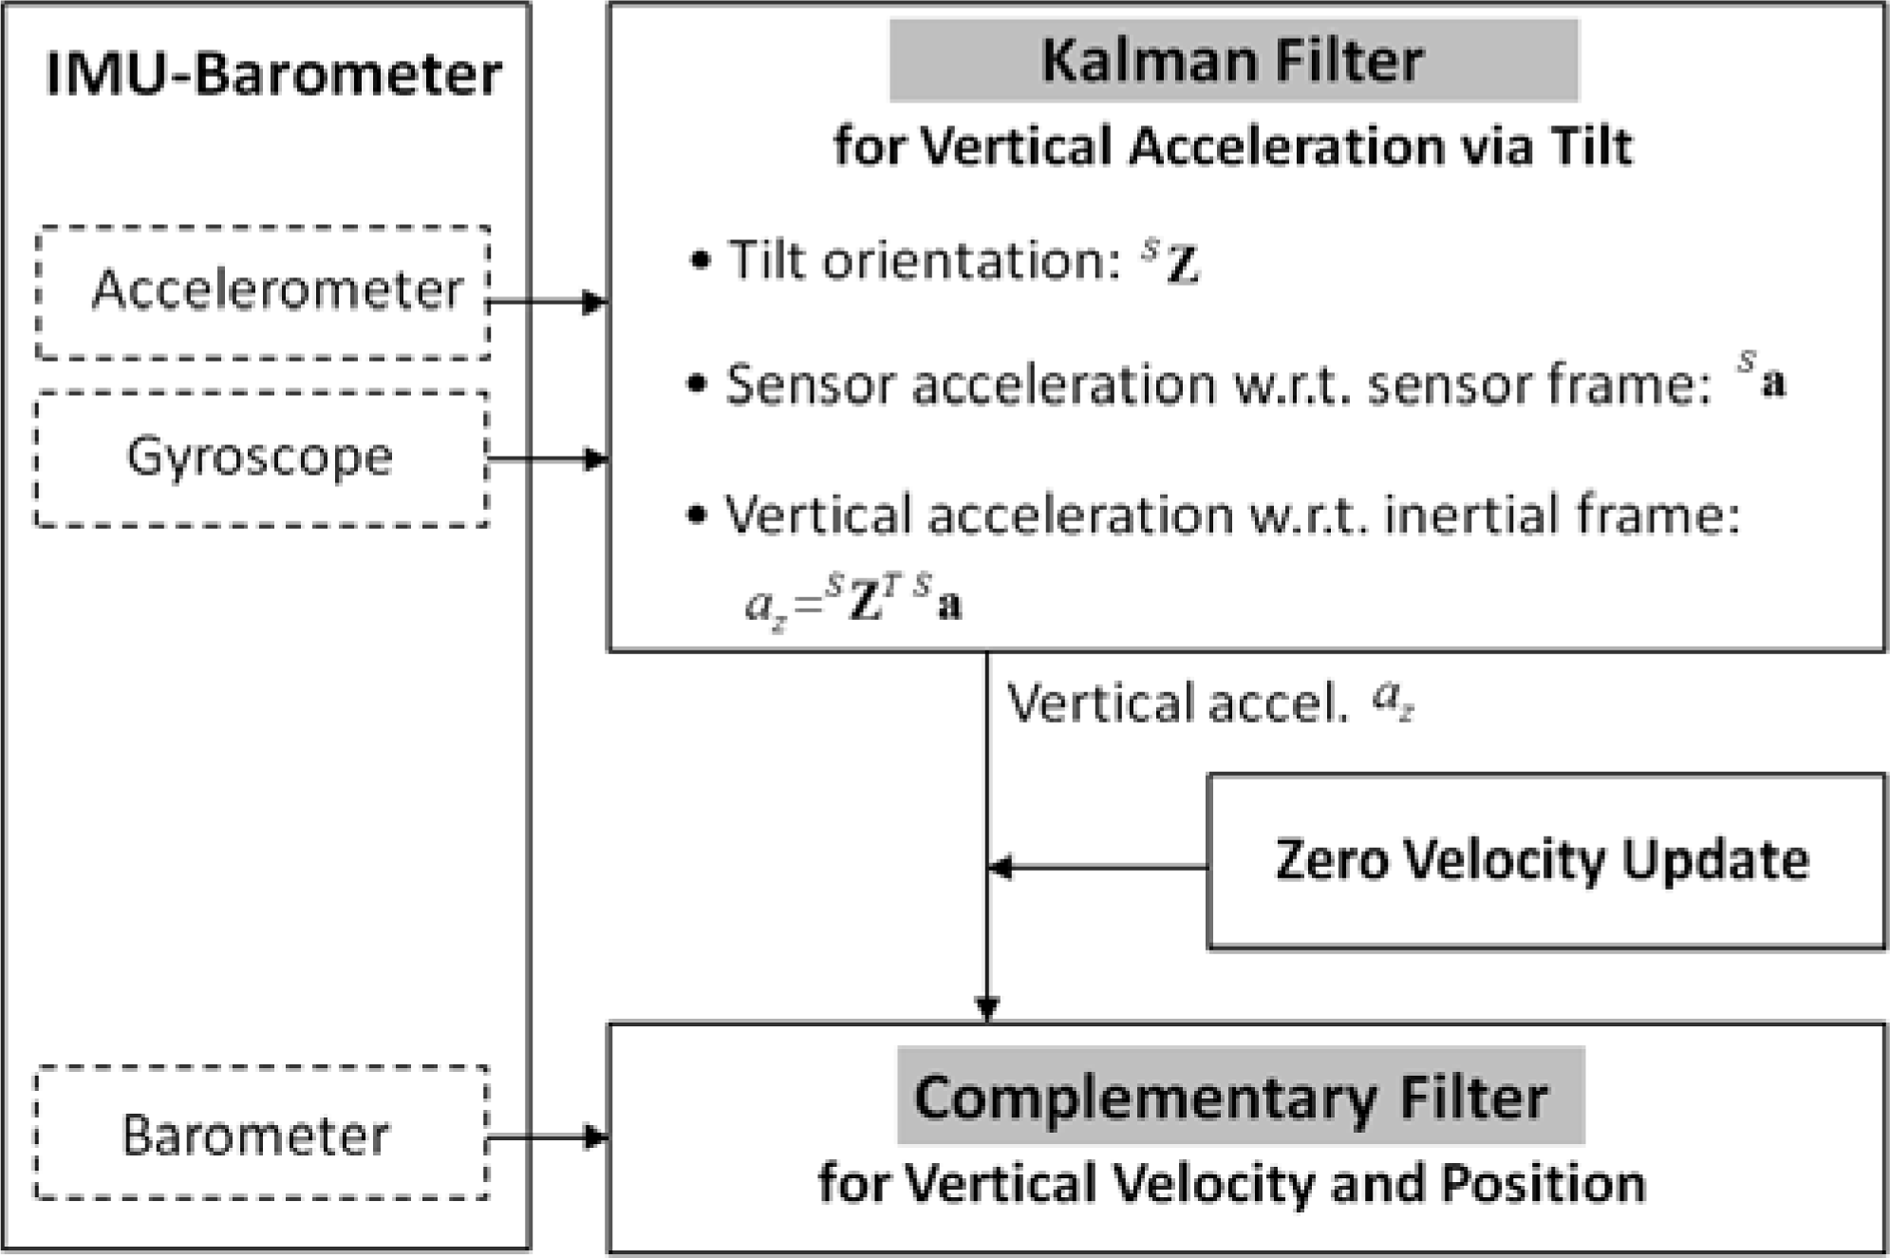
\includegraphics[width=2.5in]{fig1}
    \caption{Flowchart of the proposed two-step Kalman/complementary filter.}
\label{fig1}
\end{figure}

\begin{figure}[!t]
\centering
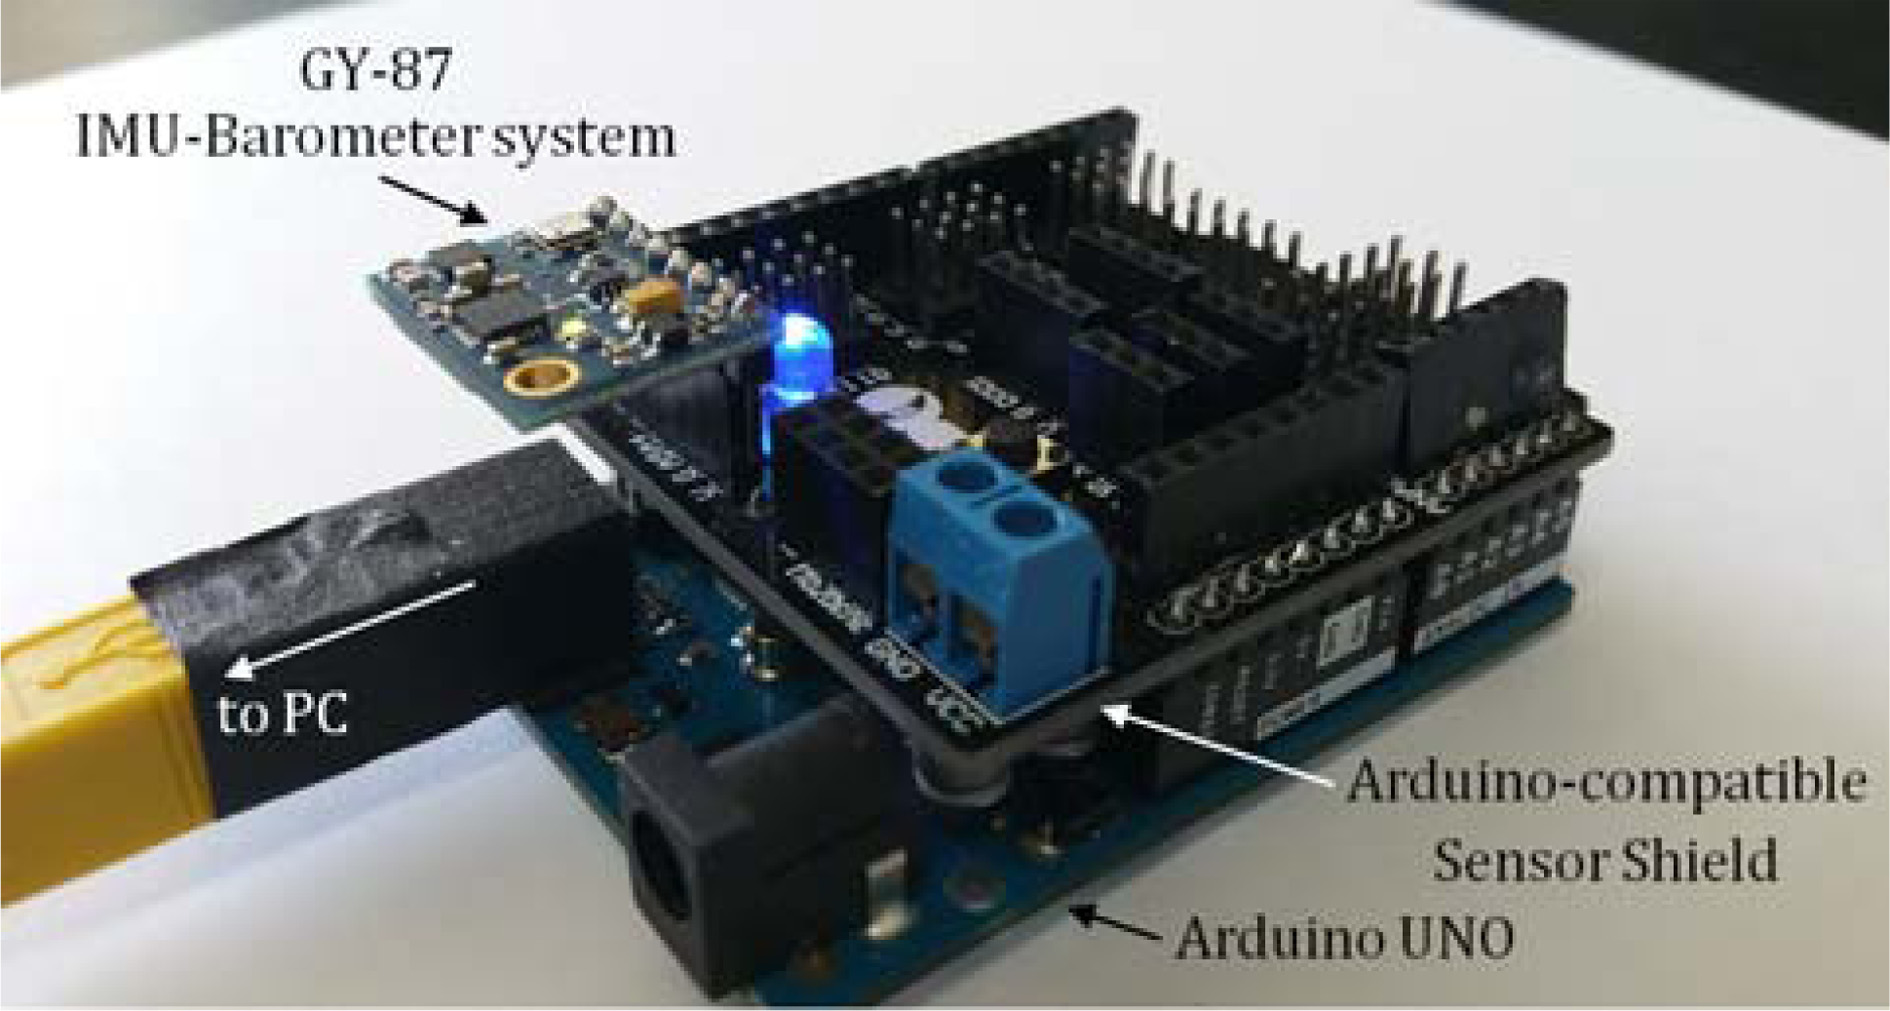
\includegraphics[width=2.5in]{fig2}
\caption{GY-87 IMU-Barometer and Arduino board system.}
\label{fig2}
\end{figure}

\begin{figure}[!t]
\centering
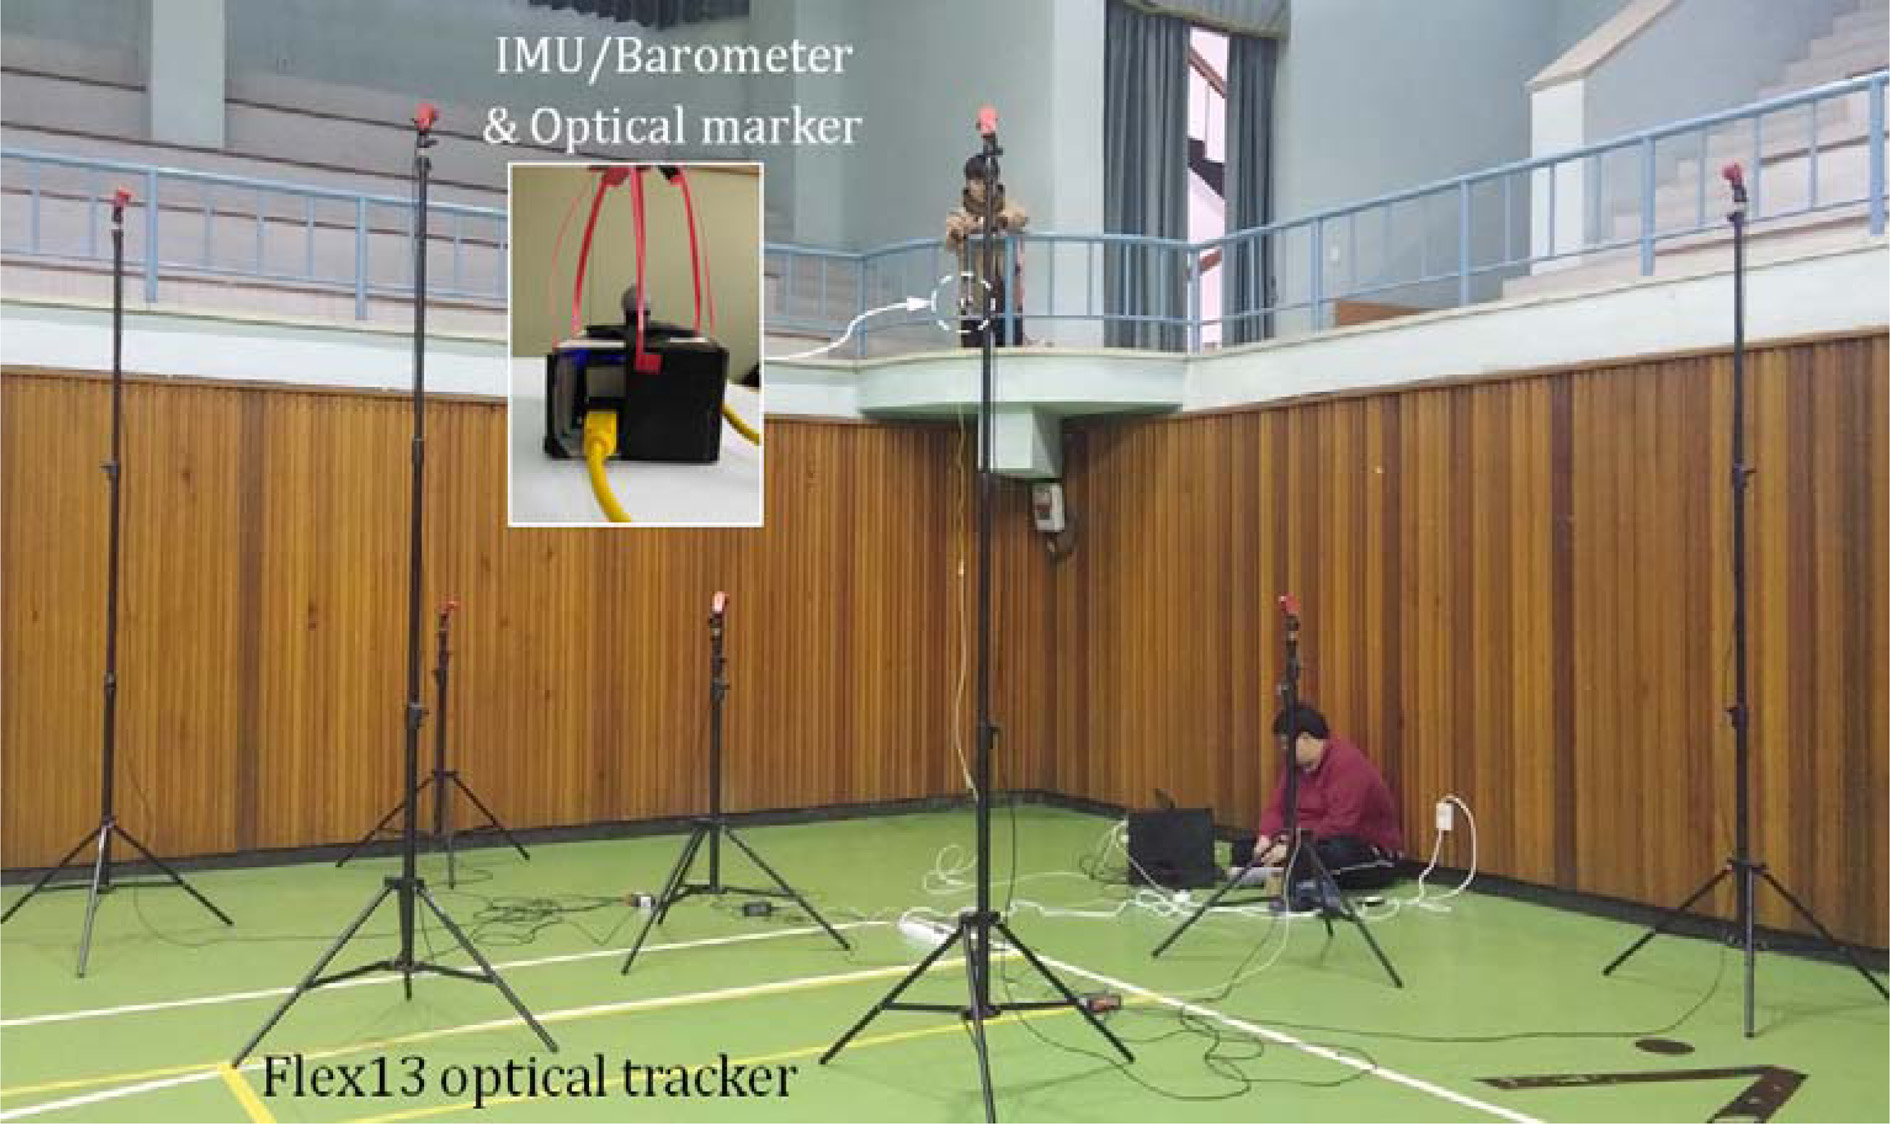
\includegraphics[width=2.5in]{fig3}
\caption{Test setup with the Fex 13 optical motion capture system in an indoor gym.}
\label{fig3}
\end{figure}


\begin{table}[tp]
\caption{Specification of GYU-87 IMU-Barometer system.}
\vspace*{-5mm}
\label{table:levels}
\centering
\begin{tabular}{llll}
\\ \toprule
& Accelerometer & Gyroscope & Barometer\\ \midrule

Model 
& \multicolumn{1}{ p{1.5cm} }{\centering Invensense \\ MPU-6050} 
& \multicolumn{1}{ p{1.5cm} }{\centering Invensense \\ MPU-6050} 
& \multicolumn{1}{ p{1.5cm} }{\centering Bosch \\ BMP 180} \\
\hline\\

Full-Scale Range 
& $\pm 2 \sim 16 g$ 
& \multicolumn{1}{ p{1.5cm} }{\centering $\pm 250 \sim$ \\ 2000 deg/s} 
& \multicolumn{1}{ p{1.5cm} }{\centering $\pm 300 \sim$ \\ 1100 hPa} \\
\hline\\

Sensitivity
& \multicolumn{1}{ p{1.5cm} }{\centering $0.000061 \sim$ \\ 0.0049 g} 
& \multicolumn{1}{ p{1.5cm} }{\centering $0.0076 \sim$ \\ 0.061 deg/s} 
& \multicolumn{1}{ p{1.5cm} }{\centering 0.0015 hPa} \\
\hline\\

\multicolumn{1}{ p{2cm} }{\centering Max. Sampling\\ Rate} 
& 1000 Hz
& 8000 Hz
& 128 Hz \\
\hline\\

Digital Resolution
& 16 bit
& 16 bit
& 19 bit\\
\hline

\end{tabular}
\end{table}  

\begin{thebibliography}{1}

\bibitem{IEEEhowto:kopka}
H.~Kopka and P.~W. Daly, \emph{A Guide to \LaTeX}, 3rd~ed.\hskip 1em plus
0.5em minus 0.4em\relax Harlow, England: Addison-Wesley, 1999.

\end{thebibliography}


\end{document}
